% schéma sur l'explication du codage H.264
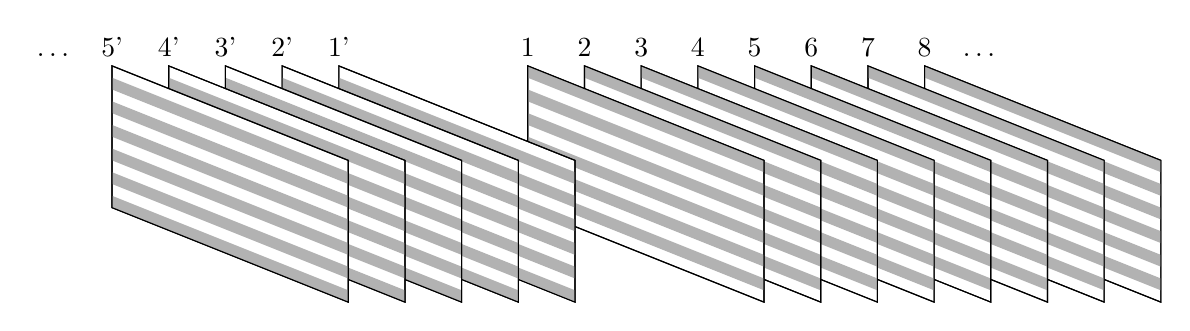
\begin{tikzpicture}[scale=0.6]
% en avant
\draw[fill=white] (18.4,0)--(23.4,-2)--(23.4,-5)--(18.4,-3) -- cycle;
\fill[fill=black!30] \foreach \i in {0,-0.5,-1,-1.5,-2,-2.5} {(18.4,-0.25+\i)--(23.4,-2.25+\i)--(23.4,-2+\i)--(18.4,\i) -- cycle};
\draw (18.4,0)--(23.4,-2)--(23.4,-5)--(18.4,-3) -- cycle;

\draw[fill=white] (17.2,0)--(22.2,-2)--(22.2,-5)--(17.2,-3) -- cycle;
\fill[fill=black!30] \foreach \i in {0,-0.5,-1,-1.5,-2,-2.5} {(17.2,-0.25+\i)--(22.2,-2.25+\i)--(22.2,-2+\i)--(17.2,\i) -- cycle};
\draw (17.2,0)--(22.2,-2)--(22.2,-5)--(17.2,-3) -- cycle;

\draw[fill=white] (16,0)--(21,-2)--(21,-5)--(16,-3) -- cycle;
\fill[fill=black!30] \foreach \i in {0,-0.5,-1,-1.5,-2,-2.5} {(16,-0.25+\i)--(21,-2.25+\i)--(21,-2+\i)--(16,\i) -- cycle};
\draw (16,0)--(21,-2)--(21,-5)--(16,-3) -- cycle;

\filldraw[fill=white] (14.8,0)--(19.8,-2)--(19.8,-5)--(14.8,-3) -- cycle;
\fill[fill=black!30] \foreach \i in {0,-0.5,-1,-1.5,-2,-2.5} {(14.8,-0.25+\i)--(19.8,-2.25+\i)--(19.8,-2+\i)--(14.8,\i) -- cycle};
\draw (14.8,0)--(19.8,-2)--(19.8,-5)--(14.8,-3) -- cycle;

\filldraw[fill=white] (13.6,0)--(18.6,-2)--(18.6,-5)--(13.6,-3) -- cycle;
\fill[fill=black!30] \foreach \i in {0,-0.5,-1,-1.5,-2,-2.5} {(13.6,-0.25+\i)--(18.6,-2.25+\i)--(18.6,-2+\i)--(13.6,\i) -- cycle};
\draw (13.6,0)--(18.6,-2)--(18.6,-5)--(13.6,-3) -- cycle;

\filldraw[fill=white] (12.4,0)--(17.4,-2)--(17.4,-5)--(12.4,-3) -- cycle;
\fill[fill=black!30] \foreach \i in {0,-0.5,-1,-1.5,-2,-2.5} {(12.4,-0.25+\i)--(17.4,-2.25+\i)--(17.4,-2+\i)--(12.4,\i) -- cycle};
\draw (12.4,0)--(17.4,-2)--(17.4,-5)--(12.4,-3) -- cycle;

\filldraw[fill=white] (11.2,0)--(16.2,-2)--(16.2,-5)--(11.2,-3) -- cycle;
\fill[fill=black!30] \foreach \i in {0,-0.5,-1,-1.5,-2,-2.5} {(11.2,-0.25+\i)--(16.2,-2.25+\i)--(16.2,-2+\i)--(11.2,\i) -- cycle};
\draw (11.2,0)--(16.2,-2)--(16.2,-5)--(11.2,-3) -- cycle;

\filldraw[fill=white] (10,0)--(15,-2)--(15,-5)--(10,-3) -- cycle;
\fill[fill=black!30] \foreach \i in {0,-0.5,-1,-1.5,-2,-2.5} {(10,-0.25+\i)--(15,-2.25+\i)--(15,-2+\i)--(10,\i) -- cycle};
\draw (10,0)--(15,-2)--(15,-5)--(10,-3) -- cycle;

\path (10,0) node[above] {1}
(11.2,0) node[above] {2}
(12.4,0) node[above] {3}
(13.6,0) node[above] {4}
(14.8,0) node[above] {5}
(16,0) node[above] {6}
(17.2,0) node[above] {7}
(18.4,0) node[above] {8}
(19.6,0) node[above] {\dots};

% en arrière
\filldraw[fill=white] (6,0)--(11,-2)--(11,-5)--(6,-3) -- cycle;
\fill[fill=black!30] \foreach \i in {-0.25,-0.75,-1.25,-1.75,-2.25,-2.75} {(6,-0.25+\i)--(11,-2.25+\i)--(11,-2+\i)--(6,\i) -- cycle};
\draw (6,0)--(11,-2)--(11,-5)--(6,-3) -- cycle;

\filldraw[fill=white] (4.8,0)--(9.8,-2)--(9.8,-5)--(4.8,-3) -- cycle;
\fill[fill=black!30] \foreach \i in {-0.25,-0.75,-1.25,-1.75,-2.25,-2.75} {(4.8,-0.25+\i)--(9.8,-2.25+\i)--(9.8,-2+\i)--(4.8,\i) -- cycle};
\draw (4.8,0)--(9.8,-2)--(9.8,-5)--(4.8,-3) -- cycle;

\filldraw[fill=white] (3.6,0)--(8.6,-2)--(8.6,-5)--(3.6,-3) -- cycle;
\fill[fill=black!30] \foreach \i in {-0.25,-0.75,-1.25,-1.75,-2.25,-2.75} {(3.6,-0.25+\i)--(8.6,-2.25+\i)--(8.6,-2+\i)--(3.6,\i) -- cycle};
\draw (3.6,0)--(8.6,-2)--(8.6,-5)--(3.6,-3) -- cycle;

\filldraw[fill=white] (2.4,0)--(7.4,-2)--(7.4,-5)--(2.4,-3) -- cycle;
\fill[fill=black!30] \foreach \i in {-0.25,-0.75,-1.25,-1.75,-2.25,-2.75} {(2.4,-0.25+\i)--(7.4,-2.25+\i)--(7.4,-2+\i)--(2.4,\i) -- cycle};
\draw (2.4,0)--(7.4,-2)--(7.4,-5)--(2.4,-3) -- cycle;

\filldraw[fill=white] (1.2,0)--(6.2,-2)--(6.2,-5)--(1.2,-3) -- cycle;
\fill[fill=black!30] \foreach \i in {-0.25,-0.75,-1.25,-1.75,-2.25,-2.75} {(1.2,-0.25+\i)--(6.2,-2.25+\i)--(6.2,-2+\i)--(1.2,\i) -- cycle};
\draw (1.2,0)--(6.2,-2)--(6.2,-5)--(1.2,-3) -- cycle;

\path (6,0) node[above] {1'}
(4.8,0) node[above] {2'}
(3.6,0) node[above] {3'}
(2.4,0) node[above] {4'}
(1.2,0) node[above] {5'}
(0,0) node[above] {\dots};

\end{tikzpicture}
